\chapter{Enjoy the Walk: Skills, People, and Future Return}

The source interview is from School of Hard Knocks and is curated here by LazyingArt LLC through Video2Book. The question is narrow: what was the most important thing learned from becoming an author? The answer is broader. The speaker does not turn first to publishing tactics, book sales, or literary craft. He uses the book's working title, "Enjoy the Walk" or "Enjoy the Journey," to explain a career mechanism: the work we are doing now matters because it leaves behind skills, people, mentors, and a record of helping others.

\section{The Question Behind Authorship}

The interviewer begins with the obvious doorway into the subject: what did the author learn from being an author? We should keep that frame in place because the answer is not simply about the book. The book becomes an occasion for a more general judgment about how careers actually accumulate value.

A thin reading would turn the answer into a slogan about enjoying the process. A more useful reading is sharper. The speaker is asking us to separate the visible product from the invisible assets produced along the way. The book is visible. The career learning, the mentors, and the relationships are the durable residue.

\section{Enjoy the Walk}

The original working title was "Enjoy the Walk" or "Enjoy the Journey." That phrase is not decorative. It tells us where to look for the value. The walk is where the skills are learned, where the people are met, and where the habits of contribution are formed.

In a formal model we might be tempted to call the job or the company the main variable. The interview pushes against that. The job and the company are locations. They are places where the more portable things can be made.

\[
\text{career value} \neq \text{job title} + \text{company name}.
\]

That displayed line is not a formula from the interview. It is a compact way of preserving the speaker's contrast. The claim is qualitative: the title and the institution are not nothing, but they are not the deepest explanation of what lasted.

\section{Looking Back While Still Looking Forward}

The speaker gives the answer from a particular vantage point. At 63, he is still looking ahead to "super exciting stuff" as an investor and a board member. That matters because the reflection is not retirement nostalgia. He is still active, but he is using hindsight to sort the durable assets from the temporary stations.

Looking back, he says that the skills he learned and the people he met along the way were what really mattered and changed his life. The order is important. First comes the journey metaphor. Then comes the retrospective test. Only then does he name the durable assets.

\begin{definition}
In these notes, the term \emph{journey capital} means the set of portable assets produced while doing the work: learned skills, trusted relationships, mentors, and a history of helping others. This is an editorial bookkeeping term, not a phrase from the interview.
\end{definition}

With that caveat, the interview's mechanism can be written as a set update rather than a financial formula:

\[
\Delta \mathcal{J}_t
=
\{\text{skills learned at }t\}
\cup
\{\text{people and mentors met at }t\}
\cup
\{\text{help given at }t\}.
\]

\[
\mathcal{J}_{t+1}
=
\mathcal{J}_t \cup \Delta \mathcal{J}_t.
\]

Here \(\mathcal{J}_t\) is not money and not a score. It is just a disciplined notation for what the speaker says remained valuable when he looked back.

\section{Jobs, Companies, and What Remains}

The interview then makes its cleanest contrast. It is not the job that you have, and it is not the company you work for. Those things may matter in ordinary ways, but they are not where the speaker places the central weight. He points instead to great mentors, great people, and the work of caring about the people around you.

\subsection{Question \& Answer}

\paragraph{Question.}
If the job and the company are not the main thing, what is?

\paragraph{Answer.}
The main thing is what can travel beyond that job and that company: the skills learned, the mentors found, the people worked with, and the pattern of helping others get better. The speaker's answer is not anti-company and not anti-career. It is a warning against mistaking the container for the contents.

We can summarize the contrast this way:

\[
\text{durable career value}
\approx
\text{skills}
+
\text{people}
+
\text{mentorship}
+
\text{help given}.
\]

The approximation sign is deliberate. This is not a measurable equation. It is a compact note-taking device for a qualitative business claim.

\section{A Simple Mechanism of Return}

The practical mechanism is reciprocal. The speaker says to care about the people you work with, help them get better, help them move up, and help them be successful even when their path later moves outside your role. That final phrase matters. The return is not confined to an org chart. The relationship can outlive the role.

\begin{figure}
\centering
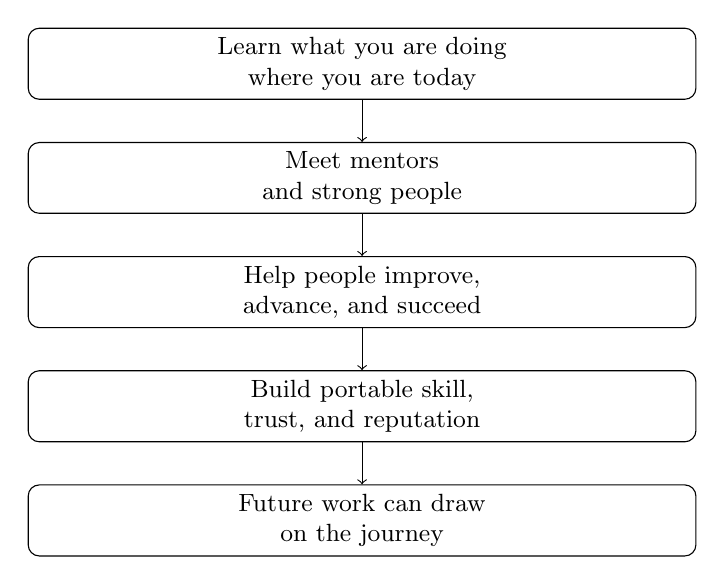
\begin{tikzpicture}[x=1cm,y=1cm,every node/.style={font=\small}]
\node[draw,rectangle,rounded corners,align=center,text width=.68\linewidth] (a) at (0,0) {Learn what you are doing\\where you are today};
\node[draw,rectangle,rounded corners,align=center,text width=.68\linewidth] (b) at (0,-1.45) {Meet mentors\\and strong people};
\node[draw,rectangle,rounded corners,align=center,text width=.68\linewidth] (c) at (0,-2.90) {Help people improve,\\advance, and succeed};
\node[draw,rectangle,rounded corners,align=center,text width=.68\linewidth] (d) at (0,-4.35) {Build portable skill,\\trust, and reputation};
\node[draw,rectangle,rounded corners,align=center,text width=.68\linewidth] (e) at (0,-5.80) {Future work can draw\\on the journey};
\draw[->] (a) -- (b);
\draw[->] (b) -- (c);
\draw[->] (c) -- (d);
\draw[->] (d) -- (e);
\end{tikzpicture}
\caption{A transcript-derived reconstruction of the speaker's mechanism. The diagram is not frame-backed; it is a compact version of the spoken sequence.}
\end{figure}

\subsection{Worked Example: Today's Role}

Suppose a person is in a present role \(R_t\). The speaker's rule is not to dismiss that role because it is not the final destination. The role can still produce the assets that matter later.

\begin{enumerate}
\item The role gives a field of practice:
\[
R_t \leadsto s_t,
\]
where \(s_t\) stands for a skill learned in the present work.

\item The same role gives contact with people:
\[
R_t \leadsto p_t,
\]
where \(p_t\) stands for a mentor, peer, colleague, or other durable relationship.

\item The role also gives chances to help:
\[
R_t \leadsto h_t,
\]
where \(h_t\) stands for help given to someone else's progress.

\item The journey capital update is then:
\[
\mathcal{J}_{t+1}
=
\mathcal{J}_t \cup \{s_t,p_t,h_t\}.
\]
\end{enumerate}

The point of the notation is limited but useful. We do not know the exact future use of \(s_t\), \(p_t\), or \(h_t\). The interview's claim is that these are precisely the kinds of things that later come back and help.

\section{Learn and Enjoy Today}

The closing advice is direct: learn what you are doing where you are today, enjoy what you are doing today, and it will come back and help you in the future. This resolves the opening question. The most important lesson from authorship is not stated as a publishing tactic. It is a rule for how to inhabit the present stage of a career.

The word "enjoy" should not be weakened into mere pleasure. In the logic of the answer, enjoying the work means staying engaged enough to learn it, notice the people around it, and contribute to them while the opportunity is present.

\section{Summary}

The chapter's central claim is that the journey is productive. A job and a company may be important settings, but the lasting assets are the skills learned, the mentors and people encountered, and the help given to others. The speaker's answer begins with authorship, moves through a retrospective career view, rejects the surface explanation of job and company, and ends with a rule for today: learn the work, enjoy the work, and let the accumulated journey become future leverage.